\chapter{CoAP-sensormodule} \label{sensormodule}

Nu we genoeg kennis hebben over Drupal en CoAP en een CoAP-\textit{library} ter beschikking hebben, kunnen we overgaan tot de uiteindelijk te ontwikkelen module. Het is deze module die een eindgebruiker zal installeren. Ze biedt dan de mogelijkheid om op een gebruiksvriendelijke en dynamische manier sensoren te bekijken en beheren van op de Drupal-website, en dit zonder technische kennis nodig te hebben van CoAP of programmatie in PHP voor Drupal. We bekijken eerst globaal wat de module concreet moet aanbieden. Daarna bekijken we hoe de module zal opgebouwd worden en welke de principes zijn waar we veel belang aan moeten hechten bij de ontwikkeling. Eens we dit weten, kunnen we overgaan tot de verschillende versies van de ontwikkelde module en de implementatie ervan. Verder bespreken we de ingevoerde databanktabellen en de nieuwe contenttypes. Als laatse onderdeel bespreken we de implementatie van de CoAP-\textit{library}\textit{hooks}.

\section{Functionaliteit}

Het doel van deze module is de eindgebruiker in staat te stellen om gemakkelijk sensoren te beheren op zijn/haar website. Belangrijk hierbij is dat elke Drupal-gebruiker die een website maakt, deze kan gebruiken zonder extra kennis nodig te hebben over CoAP. Ook is het niet de bedoeling dat de eindgebruiker nog moet programmeren om de module te kunnen gebruiken. Kortom, de module moet out-of-the-box werken en zoveel mogelijk omvatten wat mogelijk is met CoAP-sensoren.\\
%Concreet houdt dit onder andere in dat bij installatie van de module enkele contenttypes mee worden ge\"{i}nstalleerd. Het betreft hier een contenttype voor een enkele CoAP-resource en een contenttype voor een CoAP-\textit{device} waarop meerdere resources aangesloten zijn. De resources worden bij een CoAP-\textit{device} aangegeven onder vorm van het contenttype CoAP-resource. Deze contenttypes zorgen ervoor dat de gebruiker slechts met enkele muisklikken resources en \textit{devices} kan toevoegen en onmiddellijk kan beginnen met het beheren en bevragen van de resources. Verder worden bij installatie ook alle benodigde databanktabellen gecre\"{e}erd.\\

Wanneer de gebruiker een resource of een \textit{device} wil toevoegen, hoeft die enkel de URI van de resource of het IP-adres van het \textit{device} op te geven. Bij het toevoegen van een resource worden de gegevens van die resource automatisch opgehaald. En bij het toevoegen van een \textit{device}, worden de resources die zich in de well-known/core van het \textit{device} bevinden automatisch opgehaald. De gebruiker hoeft geen idee te hebben over hoe dit gebeurt.
%Deze bestaat uit het IPv6-adres van het \textit{device} waar de resource zich op bevindt en de naam van de resource, gescheiden door een '/'.
%De module zal aan de hand van een specifieke resource \textit{discovery}, de overige informatie en parameters van de resource ophalen en opslaan in de databank (Zie paragraaf \ref{resourceDiscovery}).\\
%Bij het toevoegen van een \textit{device}, hoeft de gebruiker net zoals bij een resource de URI van het \textit{device} op te geven. De informatie van de resources die zin in de well-known/core van het \textit{device} bevinden, worden automatisch opgehaald bij het toevoegen van dat \textit{device}.
%De configuratie die de gebruiker moet doen zoals bijvoorbeeld het toevoegen van een resource, moet gebruiksvriendelijk verlopen. Hiervoor wordt gebruik gemaakt van resource \textit{discovery}. In het geval van een CoAP-\textit{device} hoeft de gebruiker enkel het IPv6-adres ervan op te geven. Aan de hand van resource \textit{discovery} wordt dan een lijst gegenereerd van resources. Wanneer de gebruiker op een resource klikt, krijgt die een visuele representatie van het contenttype CoAP-resource.\\

Eens de gebruiker de gewenste resources heeft toegevoegd aan zijn/haar website, is het de bedoeling dat de 4 REST-methodes GET, PUT, POST, DELETE kunnen uitgevoerd worden. De gebruiker zal ervan op de hoogte gebracht worden wanneer een methode niet ondersteund wordt. Naast deze methodes kan een resource ook nog observable zijn (zie hoofdstuk \ref{CoAP}), de gebruiker moet dus ook in staat gesteld worden om notificaties te ontvangen van een resource. Ook wanneer een gebruiker de website verlaat moet het mogelijk zijn de \textit{observe} te laten doorlopen.

Een gebruiker moet ook gepersonaliseerde lijsten kunnen samenstellen van verschillende resources en/of \textit{devices}.

\section{Architectuur}
In deze paragraaf bespreken we de architectuur van de module en hoe die inpast in het Drupal-systeem. We behandelen tevens ook enkele belangrijke aspecten die in rekening werden gebracht. %Vervolgens lichten we enkele belangrijke onderdelen van de module toe.\\

\subsection{Requestproces}
Het proces voor het opvragen van een resourcewaarde wordt weergegeven in figuur \ref{fig:architectuur}. De acties aangeduid met een gekleurd bolletje gebeuren altijd bij een \textit{request}, de acties aangeduid met een leeg bolletje zullen pas gebeuren wanneer geen geldige waarde uit de databank kan worden gehaald (Zie paragraaf \ref{caching}). We overlopen de opeenvolgende stappen:
\begin{enumerate}
\item De browser van de \textit{client} start een \textit{request} naar de webserver waarop Drupal draait. Deze poll gebeurt onder vorm van een AJAX \textit{call}.
\item De CoAP-sensormodule voert een query uit op de databank om een geldige waarde op te vragen indien die aanwezig is.
\item De databank stuurt een resultatenset terug die een geldige waarde bevat, of leeg is indien er geen geldige waarde meer is.
\item In deze stap zijn er twee mogelijkheden:
\begin{itemize}
\item Indien er een geldige waarde aanwezig is in de databank, wordt deze teruggestuurd naar de client als antwoord op de AJAX call. De \textit{request} eindigt dan hier.
\item Indien er geen geldige waarde aanwezig is in de databank, wordt een beroep gedaan op de CoAP-\textit{library}module om een nieuwe waarde op te vragen aan de resource. 
\end{itemize}
Dit mechanisme zorgt ervoor dat de sensor niet onnodig belast wordt (Zie paragraaf \ref{caching}).
\item De CoAP-\textit{library}module stuurt een CoAP-GET-\textit{request} naar de resource.
\item De resource stuurt zijn waarde terug in een responsebericht als antwoord op de GET-\textit{request}.
\item De CoAP-\textit{library} geeft een response-object terug en roept bovendien wordt de CoAP-\textit{library}\textit{hook} hook\_recieve\_response opgeroepen.
\item De \textit{hook} zal ervoor zorgen dat de nieuwe, ontvangen waarde opgeslagen wordt in de databank.
\item Uiteindelijk wordt de waarde ook teruggestuurd naar de client die de \textit{request} heeft gestart.
\end{enumerate}
\begin{figure}
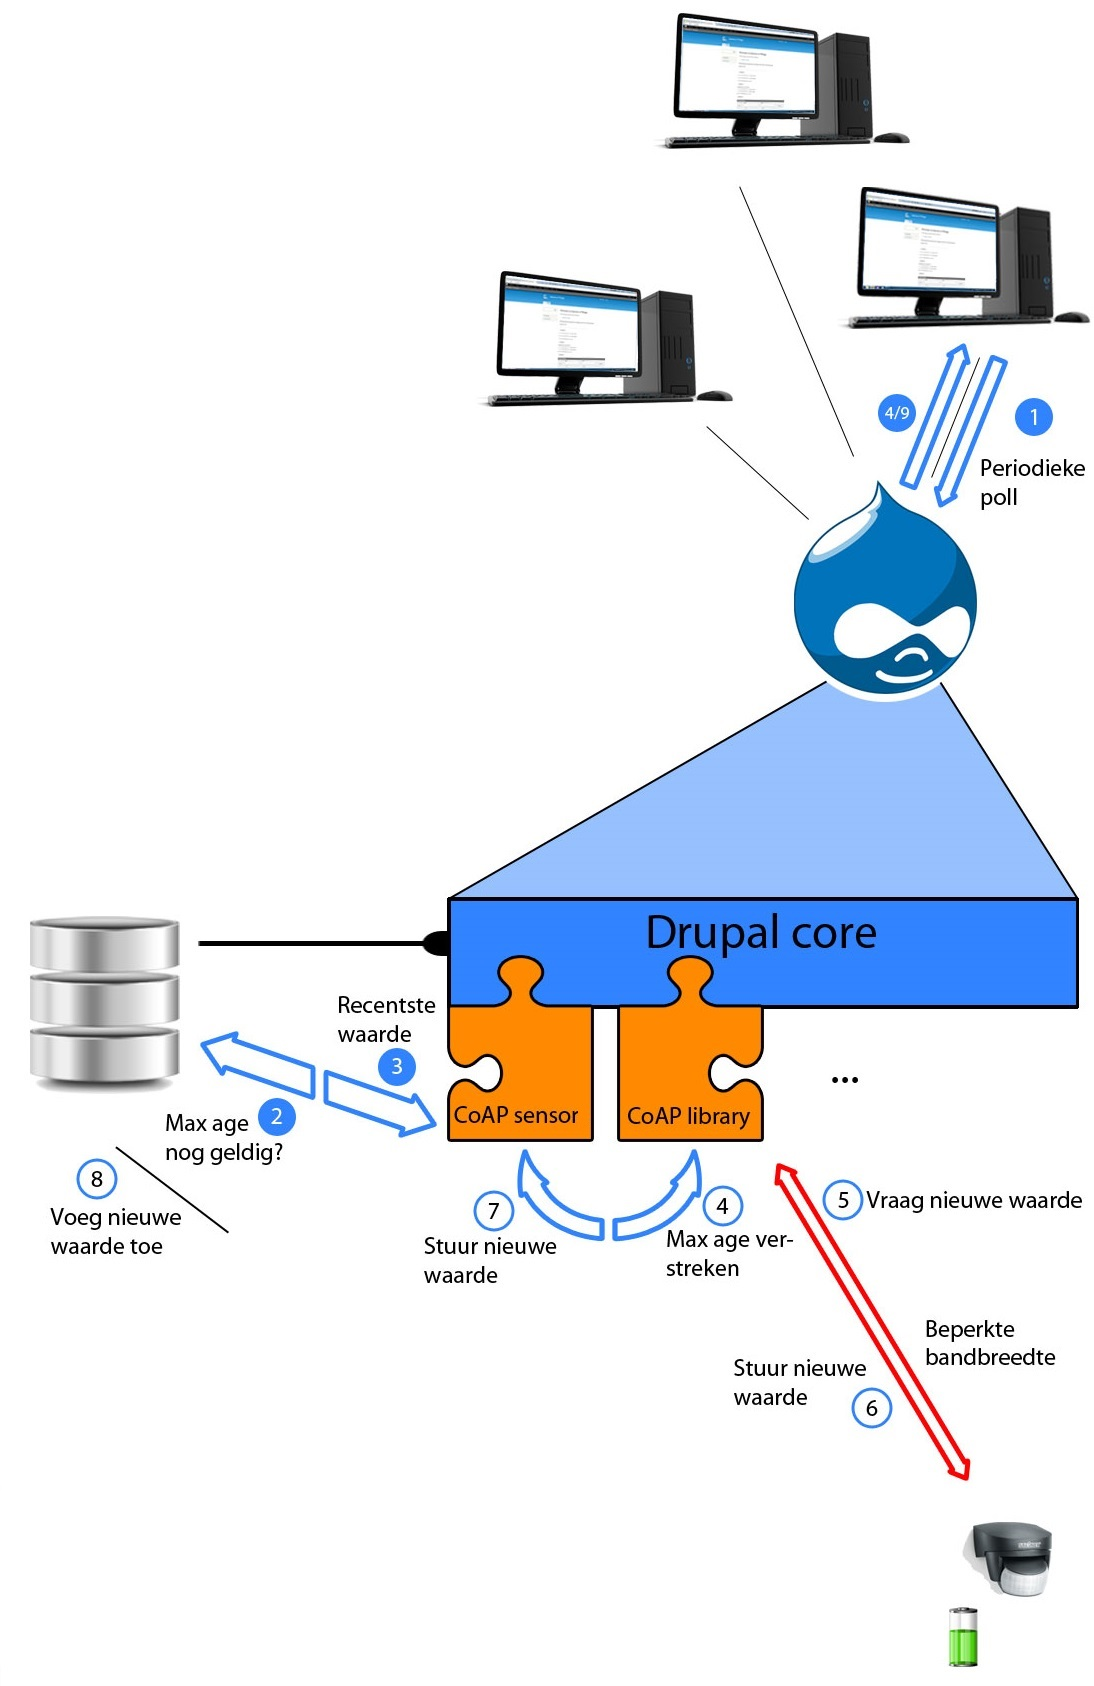
\includegraphics[width=1\textwidth]{fig/architectuur}
\caption{Resourcewaarde opvragen met de CoAP-sensormodule in Drupal}
\label{fig:architectuur}
\end{figure}

\newpage
\subsection{Belangrijke aspecten} \label{aspecten}

Deze module werd ontworpen met het oog op bepaalde aspecten waarmee rekening moet worden gehouden. We sommen enkele van de belangrijkste op.

\subsubsection{Modulariteit}
Een van de grote troeven van Drupal is de modulariteit die aangeboden wordt. Het is dan ook van uiterst belang dat onze module dit principe niet verbreekt, maar juist doorzet. In hoofdstuk \ref{coaplibrary} zagen we al hoe een aparte CoAP-\textit{library} ontwikkeld werd. Dit heeft als gevolg dat elke Drupal-gebruiker de kans heeft gebruik te maken van deze \textit{library} en dus zelf een module zou kunnen bouwen gelijkaardig aan de onze.\\
%Dit geldt ook voor deze module die we nu bespreken, deze is ook bruikbaar voor elke gebruiker die dat wil. Naast het installeren van de CoAP-\textit{library} en deze module, hoeft de gebruiker niets extra te doen om deze module te gebruiken. Databanktabellen worden gecre\"{e}erd en contenttypes worden ge\"{i}nstalleerd, zonder dat de gebruiker daar iets hoeft voor te configureren.\\
De CoAP-sensormodule maakt nog gebruik van enkele andere modules welke eerst moeten ge\"{i}nstalleerd worden door de gebruiker vooraleer hij gebruik kan maken van de CoAP-sensormodule. Drupal zal bij installatie van de CoAP-sensormodule automatisch aangeven welke modules eerst moeten worden ge\"{i}nstalleerd. Het betreft de volgende modules:
\begin{itemize}
\item \textit{Background Process} \cite{backgroundProcessModule}: Deze module maakt het gebruik van achtergrondprocessen mogelijk. (bijvoorbeeld voor \textit{observe})
\item \textit{Progress} \cite{progressModule}: Deze module moet worden toegevoegd omdat de \textit{Background Process}module hiervan afhankelijk is.
\item CoAP-\textit{library} (Zie hoofdstuk \ref{coaplibrary}): Onze eigen geschreven module die instaat voor alle CoAP-communicatie.
\item \textit{Entity API} \cite{entityApiModule}: Een veelgebruikte module (die opgenomen wordt in de core van Drupal 8). Breidt de functionaliteit uit die met entities kan verwezenlijkt worden.
\item \textit{Node reference} \cite{nodeReferenceModule}: Een module die gebruikt wordt om in een bepaalde node door middel van een veld te verwijzen naar andere nodes.
\end{itemize}

\noindent
Er zijn ook modules die niet strikt noodzakelijk zijn maar wel extra functionaliteit bieden:
\begin{itemize}
\item \textit{Views}\cite{viewsModule}: Maakt het gebruik van views mogelijk.
\item \textit{Views UI}: Stelt een \textit{user interface} ter beschikking om eigen views te maken en te beheren. Deze module is onderdeel van de viewsmodule.
\end{itemize}

\subsubsection{Minimalisatie van netwerkbelasting}
Mogelijks zijn meerdere gebruikers van een Drupal-website ge\"{i}nteresseerd in een observable resource. Het is niet aanvaardbaar dat de netwerkbelasting zou stijgen met het aantal ge\"{i}nteresseerden voor die resource. Daarom gedraagt Drupal zich eigenlijk als intermediaire server voor de eindgebruikers. Er wordt namelijk maar \'{e}\'{e}n \textit{observe} op die resource uitgevoerd door Drupal, ongeacht het aantal gebruikers dat ge\"{i}nteresseerd is in die resource. De notificaties worden op de server in de databank gestopt en het zijn deze waarden waarop de gebruikers uiteindelijk pollen. %\\
%Bovendien zorgt dit voor een vorm van controle over verkeer naar de resources, de gebruikers van de website kunnen namelijk niet zelfstandig CoAP praten met de resources. % Een voorbeeld hiervan is de demo van de module op onze website (http://www.thesisinternetofthings.tk). Enkel ingelogde gebruikers zijn in staat een \textit{observe} uit te voeren. Dit om te vermijden dat gelijk wie een \textit{observe} kan starten, men kan namelijk vergeten de \textit{observe} af te sluiten, waardoor de databank meer en meer opgevuld wordt.

\subsubsection{Asynchroniteit}
In een eerste fase van deze module werd er gebruik gemaakt van een formulier. Bij het indienen van dit formulier, werd eerst de \textit{request} om de waarde op te halen uitgevoerd en dan gewacht op de response om de nieuwe pagina op te bouwen. Het spreekt voor zich dat dit geen goede oplossing is, omdat het renderen van de pagina maar kan gebeuren nadat de response aangekomen en verwerkt is. Zo kan de gebruiker de indruk krijgen dat de verbinding met de website verbroken is wanneer de communicatie traag is of misloopt. \\

In hoofdstuk \ref{Drupal} zagen we als mogelijke oplossing het gebruik van jQuery. In deze situatie is jQuery echter geen goede optie omdat jQuery de databank van Drupal niet zonder bijkomende informatie kan manipuleren. Hiervoor zouden een connectiestring, wachtwoord en dergelijke gegevens nodig zijn. JQuery van die informatie voorzien is een grote bedreiging voor de veiligheid. Bovendien zou dit een oplossing zijn met een zeer sterke koppeling, wat nooit een goed idee is.\\
De gebruikte oplossing illustreert alweer de voordelen van een open source platform met een uitgebreide community. Er is namelijk al een \textit{Background Process}module gemaakt, het zou dus zonde zijn om hier niet dankbaar gebruik van te maken. Zoals de naam suggereert, biedt de \textit{Background Process}module de mogelijkheid om achtergrondprocessen op te starten. Deze draaien op de achtergrond op de server en storen dus geen andere processen zoals het opbouwen van een pagina voor de gebruiker. De gebruiker wordt dus niet meer geconfronteerd met lange wachttijden.\\
Sterker nog, er is ook een functie voorzien om een HTTP-GET-\textit{request} uit te voeren, waarbij je een \textit{callback}-functie opgeeft. Wanneer er een response is, zal dus automatisch de opgegeven functie als achtergrondproces opgeroepen worden met de response als argument. Deze functie zal dus goed van pas komen in de eerste versie van de module, die gebruik maakt van een HTTP/CoAP-proxy. Deze wordt beschreven later in dit hoofdstuk (Zie paragraaf \ref{proxy}).

\subsubsection{Strategie bij ontvangst van waarden}
\paragraph{Push-strategie:}

De mooiste oplossing en tevens degene met het minste aandeel aan overhead, is een oplossing waarbij de server zelf op eigen initiatief data kan sturen naar de client. Merk op dat we hier als server de Drupal-server bedoelen en als client de browser. Hierbij is dan geen \textit{polling}mechanisme nodig door de client, wat de netwerkbelasting drastisch verlaagt en de verantwoordelijkheid verschuift naar de server.\\
Om een \textit{push}-strategie te verwezenlijken werd een uitgebreide literatuurstudie van node.js uitgevoerd. Node.js is een JavaScript \textit{library} die je in staat stelt bi-directioneel verkeer te verwezenlijken. Hierbij wordt gebruik gemaakt van kanalen die worden opgezet, zo'n kanaal kan dan door beide partijen gebruikt worden.\\
Concreet zou het in de context van deze masterproef mogelijk zijn om met node.js een JavaScript-functie op te roepen bij de client op initiatief van de server.\\

Er is meermaals gepoogd dit te realiseren, maar de summiere documentatie van node.js laat op sommige vlakken te wensen over. Zo zijn we er niet in geslaagd documentatie te vinden over het opzetten van een eigen kanaal of een bestaand kanaal te gebruiken.\\
Bovendien is het nodig voor \textit{websockets}, de onderliggende technologie, om een extra server te draaien waarlangs het verkeer moet passeren. Aangezien het vaak niet mogelijk is om de shell van de webserver te gebruiken in een shared-hosting omgeving, is dit een erg groot nadeel. Er bestaan wel servers die je kan gebruiken, maar dit tegen betaling. Wij, als ontwikkelaar van de module, kunnen niet verwachten dat een eindgebruiker een extra server ter beschikking heeft of dat zelfs wil. Het is de bedoeling dat onze module zo veel mogelijk out-of-the-box bruikbaar is.\\

De conclusie is dat wij geopteerd hebben geen gebruik te maken van node.js en dus ook niet van een \textit{push}-strategie. Er zijn echter wel nog pull-mechanismen die het push-mechanisme simuleren die het vernoemen waard zijn, zoals long polling \cite{longPolling}, SSE \cite{SSE}, ...
\newpage
\paragraph{Pull-strategie: }

Aangezien een \textit{push}-strategie niet of moeilijk kan gebruikt worden, hebben wij gekozen voor een \textit{pull}-oplossing.\\

Uiteraard was de eerste reactie gebruik te maken van de Drupal-community en dus te zoeken in de vele modules die beschikbaar zijn. Er is tot op heden geen module geschreven door iemand anders in de Drupal-community dat ons probleem behandelt. De inspiratie voor de uiteindelijke oplossing werd wel gehaald uit een bestaande module, namelijk de \textit{Block Refresh}-module \cite{blockRefreshModule}.\\
Deze laatste maakt gebruik van jQuery en \textit{AJAX calls} om periodiek de inhoud van een block te refreshen, waarbij je zelf de lengte van de periode kan bepalen. In jQuery loopt een timer die periodiek een JavaScript-functie oproept. In deze functie wordt dan een \textit{AJAX call} uitgevoerd naar de Drupal-server, die op zijn beurt een antwoord terugstuurt.\\

Wij hebben geopteerd het mechanisme licht te wijzigen in plaats van de module zelf te gebruiken. Aan de basis van deze beslissing liggen drie redenen:
\begin{itemize}
\item Wij wensen de content slechts aan te passen wanneer nodig. Dit wil zeggen, wanneer een nieuwe waarde is binnengekomen. Bovendien hoeft niet alle content vernieuwd te worden, dit doet de \textit{Block Refresh}module wel.
\item De configuratie van de periode voor het vernieuwingsinterval is in onze ogen relatief omslachtig. De gebruiker moet al een configuratievenster openen om het interval te wijzigen, wat wachttijden met zich meebrengt. Het zal blijken dat in onze uiteindelijke module het interval snel en gemakkelijk te wijzigen is. 
\item De uiteindelijke module zal geen blocks meer gebruiken, maar contenttypes. Dit maakt het gebruik van de \textit{Block Refresh}module zelfs onmogelijk.
\end{itemize}

De aangepaste methode werkt als volgt: Wanneer de pagina geladen wordt bij de client, start een timer die periodiek een \textit{AJAX call} uitvoert naar de Drupal-server. De gebruiker kan hierbij bepalen hoe lang die periode moet zijn. Op de Drupal-server is dan een \textit{AJAX call}back functie gedefinieerd aan de hand van de \textit{hook} hook\_menu(). Deze \textit{hook} wordt gebruikt om menu items toe te voegen aan de site en om \textit{AJAX call}backs te definieren. Alle output die gegenereerd wordt in deze \textit{callback} wordt als antwoord teruggestuurd op de \textit{AJAX call}back.\\

Wat de \textit{callback} terugstuurt en hoe die inhoud wordt verwerkt, verschilt per versie van onze module. Dit zal dan ook besproken worden in de gepaste paragrafen (Zie paragraaf \ref{evolutie}).

\subsubsection{Caching}\label{caching}
Een bericht kan een maximum levensduur hebben, dit wordt aangegeven met een \textit{max-age}optie (optie 14) in het bericht. Deze bevat dan een numerieke waarde die aangeeft in seconden hoelang de waarde als geldig mag worden beschouwd. Wanneer deze maximum levensduur overschreden wordt, mag deze waarde niet meer worden gebruikt. Dan moet bij een volgende aanvraag door een gebruiker een nieuwe waarde worden opgehaald van de resource. Bijgevolg wordt een opgehaalde waarde in de databank gestopt. Wanneer de maximum levensduur nog niet overschreden is bij een aanvraag, wordt de waarde uit de databank gehaald. De resource en het netwerk worden dan dus niet onnodig belast. Dit zorgt er ook voor dat de belasting op een resource niet evenredig stijgt met het aantal gebruikers die er een waarde van willen opvragen.\\
Dit aspect is zeker een van de meer belangrijke omdat verbindingen naar een resource vaak een beperkte bandbreedte kennen. Bovendien bestaat de energievoorziening van sensoren vaak uit een batterij. Het werk dat zo'n sensor moet verrichten, moet dus worden geminimaliseerd.

\section{Evolutie van de module} \label{evolutie}

\subsection{Temperatuurmodule met HTTP/CoAP-proxy} \label{proxy}
In deze paragraaf wordt besproken hoe de eerste versie van de module werd gemaakt die gebruik maakt van een HTTP/CoAP-proxy. Bovendien wordt ook aangetoond hoe waarden opgeslagen worden in de databank om de geschiedenis van opvragingen bij te houden. We spreken hier (en in enkele volgende paragrafen) beter van een temperatuurmodule, aangezien deze module slechts \'{e}\'{e}n resource bevraagt. Het betreft een resource die de waarde van een temperatuursensor terugstuurt. Deze resource werd gekozen vanwege de numerieke waarde die teruggestuurd wordt en omwille van het feit dat de resource observable is.\\

De module wordt aan de gebruiker gepresenteerd onder de vorm van een Drupal-block. Dit block bevat een HTML-formulier met twee componenten die als invoer dienen. Een \textit{\textit{checkbox}} die aanduidt of de gebruiker waarden automatisch wil laten ophalen, en een knop die het formulier indient wanneer de gebruiker erop klikt.\\
Wanneer de gebruiker op de knop klikt en de \textit{\textit{checkbox}} heeft aangevinkt, worden waarden automatisch opgehaald met een interval gelijk aan de waarde van de \textit{max-age}. Merk op dat het hier nog niet om een CoAP-\textit{observe} gaat. In deze module werken we met een HTTP/CoAP-proxy. Periodiek wordt een HTTP-GET-\textit{request} naar een HTML-pagina uitgevoerd. Wanneer de response ontvangen wordt, wordt de HTML-pagina geparsed, waarna de nuttige informatie in de databank wordt geplaatst. Met jQuery worden dan nieuwe waarden periodiek opgehaald en getoond aan de gebruiker.\\

Er is bij deze versie nog geen sprake van achtergrondprocessen waardoor het lang kan duren eer een pagina geladen wordt. Bovendien krijgt de gebruiker enkel een foutmelding (van de gebruikte webserver) te zien wanneer er geen communicatie mogelijk is.

\begin{figure}[h!]
\vspace{10pt}
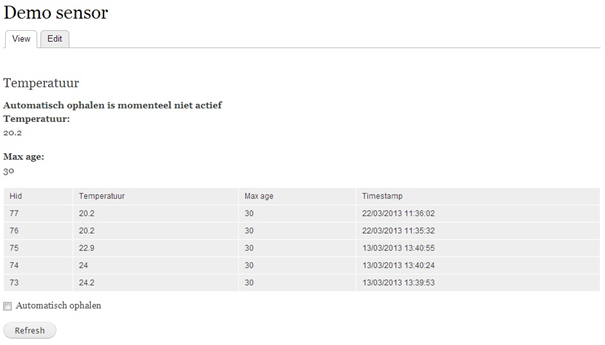
\includegraphics[width=1\textwidth]{fig/TemperatuurModuleHTTPCOAPProxy}
\vspace{-30pt}
\caption{Temperatuurmodule met HTTP/COAP-proxy}
\vspace{-10pt}
\end{figure}

\subsubsection{Proxy}
Als proxy werd de coap.me-website \cite{coapMe} gebruikt. Deze biedt de mogelijkheid om notificaties van een \textit{embedded device} te bekijken in een browser. De website biedt ook de mogelijkheid om door te klikken naar de notificatie om die volledig te bekijken op een pagina.\\

Het is deze laatste pagina die periodiek wordt opgehaald en geparsed. De communicatie vanwege de Drupal-module bestaat dus enkel uit HTTP-communicatie, de proxy verzorgt de nodige CoAP-berichten tussen zichzelf en het \textit{embedded device}.

\subsubsection{Polling}
In deze eerste versie van de module bestond het antwoord bij de \textit{polling} uit de volgende velden:
\begin{itemize}
\item Hid: De History ID dat een numeriek ID is voor de opgevraagde waarde. Het is tevens de index in de databanktabel met waarden en is dus uniek.
\item Temperatuur: Dit is de effectieve waarde in graden Celsius. Deze werd geparsed uit de responsestring afkomstig van de resource.
\item \textit{Max-age}: De antwoorden van de betreffende resource bevatten een max-ageoptie. Dit is het aantal seconden dat deze waarde als geldig mag beschouwd worden.
\item \textit{Timestamp}: Het tijdstip waarop de waarde ontvangen werd.
\end{itemize}

\subsection{Temperatuurmodule met native CoAP}
Nu de omliggende structuur opgezet en uitgetest is, kan de communicatie veranderen van HTTP-berichten naar native CoAP. Er is in deze versie echter nog geen sprake van de CoAP-\textit{library}. Deze versie beperkt zich tot een eerste test met CoAP-communicatie.\\

Voor CoAP-verkeer zal UDP gebruikt worden zoals voorgeschreven in de CoAP-draft \cite{coapDraft}. Eerst wordt een UDP-socket geopend naar het betreffende IPv6-adres van het \textit{embedded device} waarop de resource is aangesloten. Dit gebeurt met de functie pfsockopen() van PHP, deze opent een persistente socket. Vervolgens wordt een hexadecimale string opgesteld die het bericht voorstelt. Ook deze opstelling gebeurt aan de hand van de CoAP-draft \cite{coapDraft}. Het bericht wordt verstuurd met de fwrite() functie. Hierna kan het antwoord opgehaald worden van de socket met de fread() functie die als enige parameter een grootte in bytes verwacht. Belangrijk hierbij is dat de opgegeven grootte minstens even groot is als het aantal bytes van het volledige antwoord.\\

\subsubsection{Observe}
Nu er gebruik gemaakt wordt van native CoAP, is er ook een echte CoAP-\textit{observe} mogelijk. Hierbij is het noodzakelijk dat de socket opengehouden wordt. Dit omdat het \textit{embedded device} nu op eigen initiatief berichten kan sturen. Aangezien de socket moet worden opengehouden, kan de code niet meer op de voorgrond draaien. Indien dit wel zo zou zijn, zou de pagina nooit gerenderd worden. De gebruiker zou dan geconfronteerd worden met een timeout van de webserver waarop Drupal draait. Achtergrondprocessen zijn nu dus geen optie meer, maar een noodzaak. De code om een socket open te houden en te beheren zal dus opgestart worden in een achtergrondproces aan de hand van de \textit{Background Process}module die eerder al vermeld werd \cite{backgroundProcessModule}.\\
Bij ontvangst van een notificatie van de CoAP-resource zal de waarde in de databank worden gestopt met bijbehorende velden. Deze velden zijn dezelfde als in de vorige versie van de module (Zie paragraaf \ref{proxy}). Het zijn deze waarden waarop de client met jQuery zal pollen. Ook deze \textit{polling} gebeurt op dezelfde manier als in de vorige versie van de module.

\subsection{CoAP-sensormodule met externe CoAP-library}
Alle code die te maken had met CoAP-communicatie was hardgecodeerde code wat onvermijdelijk leidde tot duplicatie van code. Bovendien bevond deze code zich in dezelfde module als diegene die nu wordt besproken. Dit heeft als gevolg dat andere gebruikers van Drupal geen gebruik kunnen maken van onze code om CoAP-berichten te sturen en te ontvangen. Dit alles heeft geleid tot de ontwikkeling van onze eigen CoAP-\textit{library} in PHP onder de vorm van een externe module die apart kan worden gebruikt. Deze \textit{library} werd eerder al besproken in hoofdstuk \ref{coaplibrary}.\\

\subsubsection{Nieuwe block}
De module onderging in deze stap naast een visuele verbetering, ook een verbetering van functionaliteit (Zie figuur \ref{fig:meerdereResources}). Zo kan de gebruiker nu met \'{e}\'{e}n block meerdere resources bevragen.\\

De gebruiker kan \'{e}\'{e}n resource selecteren met \textit{radiobuttons}, wanneer de gebruiker dan op de knop 'Bekijken' klikt, wordt de pagina herladen en is de geselecteerde resource te bevragen. Door op de knop 'GET' te klikken, wordt een GET-\textit{request} uitgevoerd op de geselecteerde resource.\\
Er wordt ook een lijst met \textit{checkboxes} ter beschikking gesteld. De gebruiker kan hierbij de resources aanvinken waarop een \textit{observe} moet worden uitgevoerd. Wanneer de gebruiker een aangevinkte \textit{checkbox} uitvinkt, zal de \textit{observe} stoppen. De instellingen worden opgeslagen en de benodigde acties worden uitgevoerd wanneer de gebruiker op de knop 'Observe' klikt. Belangrijk hierbij is dat wanneer de pagina herladen wordt, de juiste \textit{checkboxes} al worden aangevinkt zodat de gebruiker ten allen tijde weet welke resources al geobserveerd worden.\\
Een laatste verbetering bestaat uit een grafiek die automatisch wordt gegenereerd op basis van de geschiedenis van opvragingen. De grafiek wordt aan de hand van een \textit{AJAX call} en de \textit{Google Charts API} \cite{googleCharts} gerealiseerd. Het betreft hier de waarden van de resource die momenteel bekeken wordt en dus aangeduid is met een \textit{radiobutton}.

\begin{figure}[h!]
\centering
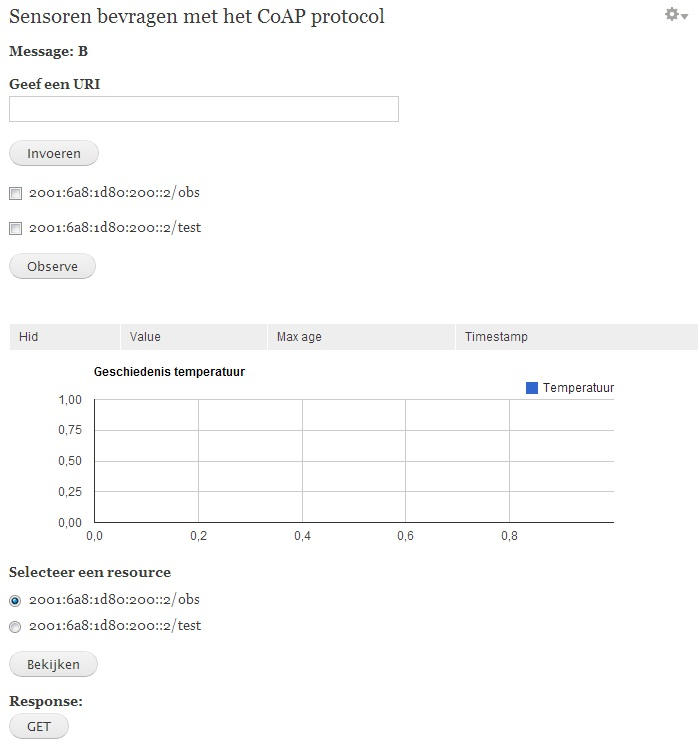
\includegraphics[width=1\textwidth]{fig/meerdere_resources}
\caption{Block met HTML-formulieren die de gebruiker toelaat meerdere resources met \'{e}\'{e}n block te bevragen}
\label{fig:meerdereResources}
\end{figure}

\subsection{CoAP-sensormodule met contenttype CoAP-resource}
In de vorige versies werd de module weergegeven aan de hand van een HTML-formulier in een Drupal-block. Het nadeel hiervan is dat men standaard slechts \'{e}\'{e}n instantie van het block gebruikt. Men kan echter wel het een en het ander verbeteren met de \textit{Views}module, maar het is niet de bedoeling dat wij dit verlangen van de gebruiker. Bovendien is een block slechts een visuele blok op de website, het is niet echt een node of een stuk content.\\

Een beter en vaak gebruikt alternatief is het maken van een eigen contenttype. Wanneer men nu deze module installeert worden de contenttypes gedefin\"{i}eerd in de module, mee ge\"{i}nstalleerd. Dit heeft als gevolg dat de gebruiker slechts op 'Add content' hoeft te klikken (Zie figuur \ref{fig:addContent}), enkele benodigde velden in moet vullen en de content wordt automatisch gegenereerd en opgeslagen. Bij deze methode wordt al deze configuratie afgehandeld door Drupal-mechanismen, zo worden bijvoorbeeld de velden opgeslagen in tabellen die behoren tot de Drupalcore. Dit betekent dat onze content effectief wordt ingepast en geen losstaand geheel is. Het beheer van de content, manipulatie en dergelijke zal dus gebeuren met Drupal zoals dat gebeurt voor andere contenttypes. We merken ook op dat wanneer een resource verwijderd wordt, dit niet het geval is voor de waarden die ervan opgehaald zijn. Deze blijven aanwezig in de databank en zullen ook weer te zien zijn wanneer de resource later opnieuw wordt toegevoegd.\\

\subsection{CoAP-sensormodule met volledige REST-functionaliteit} \label{rest}
Tot nog toe was enkel een GET-\textit{request} mogelijk naar een resource, maar vaak ondersteunt een resource ook nog andere REST methodes (GET, PUT, POST, DELETE). Het is dus van groot belang dat onze module ook de mogelijkheid biedt om alle REST methodes uit te voeren.\\

Dit brengt ook mee dat de visuele representatie zal wijzigen (Zie figuur \ref{fig:rest}). De vier methodes worden met knoppen weergegeven in een tabel, eventueel vergezeld van een tekstveld indien invoer vereist is (PUT en POST). Onderaan de tabel wordt de response en response method (205 Content, 405 Bad method,...) getoond.\\
Wij hebben ervoor gekozen dat de gebruiker voor elke resource, op elk moment elke REST methode kan uitvoeren. Er wordt namelijk al een gepaste response getoond wanneer een methode niet ondersteund is. Bovendien is een server niet verplicht in een resource \textit{discovery} (Zie paragraaf \ref{resourceDiscovery}) aan te geven welke methodes ondersteund zijn. Wil men voor elke resource toch methodes uitschakelen die niet ondersteund zijn, dan zou men elke methode eens moeten uitproberen en verif\"{i}eren of een 405 Bad Request teruggestuurd wordt.

\begin{figure}[h!]
\centering
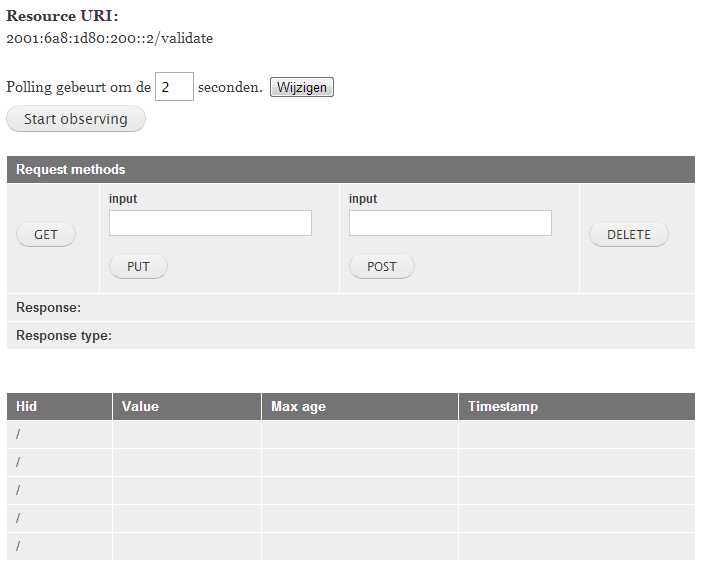
\includegraphics[width=1\textwidth]{fig/rest}
\caption{CoAP-resource met volledige REST functionaliteit}
\label{fig:rest}
\end{figure}

\subsection{CoAP-sensormodule met resource discovery}
De gebruiker is nu in staat meerdere CoAP-resources toe te voegen aan zijn/haar website. Het kan echter moeilijk zijn een overzicht te behouden over al deze resources en bovendien moet men van elke resource de specifieke URI kennen, wat zeker niet vanzelfsprekend is.\\

Deze nadelen kunnen worden weggewerkt door gebruik te maken van het concept resource \textit{discovery}. De technische uitleg en implementatiedetails werden al besproken in paragraaf \ref{resourceDiscovery}. In deze module krijgt de gebruiker na het uitvoeren van een resource \textit{discovery}, een lijst van CoAP-resources te zien die aangesloten zijn op het \textit{embedded device}. Om performantieredenen en omwille van het feit dat een well-known/core weinig of nooit verandert, wordt het resultaat van de resource \textit{discovery} (Zie paragraaf \ref{resourceDiscovery}) opgeslagen in de databank. De manier waarop de gegevens opgeslagen zijn is dezelfde als in het eindresultaat en wordt besproken in \ref{databankSchema}. Er wordt echter op de website wel nog een Refresh-knop voorzien mocht de gebruiker de gegevens in de databank toch willen vernieuwen.\\
Op de website wordt een resource weergegeven door de URI en door de \textit{human readable name}. Bovendien is voor elke resource ook een \textit{checkbox} voorzien om aan te duiden dat de gebruiker ge\"{i}nteresseerd is in de resource. De gekozen resources worden dan opgesomd en ter beschikking gesteld op dezelfde manier als in de vorige versie van de module (Zie figuur \ref{fig:meerdereResources}). In de volgende twee subparagrafen bespreken we twee mogelijke vormen die wij gemaakt hebben om de resource \textit{discovery} en opsomming van de resources te combineren.

\begin{figure}[h!]
\centering
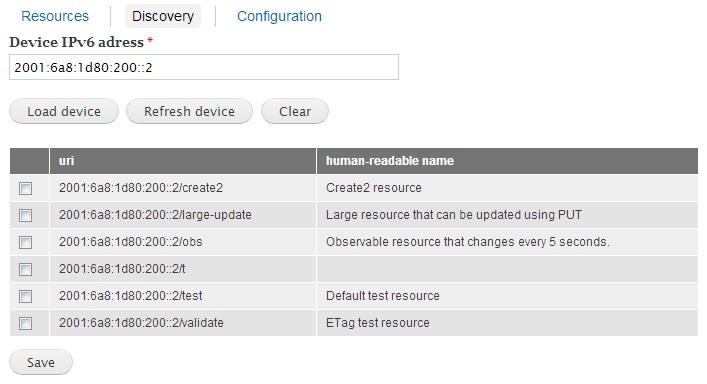
\includegraphics[width=1\textwidth]{fig/tabbladen}
\caption{Opsomming van resources aan de hand van resource discovery}
\label{fig:tabbladen}
\end{figure}

\subsubsection{Multi-form}
Een eerste mogelijkheid bestaat erin eerst de lijst te presenteren aan de gebruiker. De gebruiker kiest dan een aantal resources die hij/zij wil toevoegen aan de website, waarna hij/zij op de knop 'Save' klikt. Hierna wordt een nieuwe pagina getoond die de gebruiker toelaat de resources te beheren en te bevragen (Zie figuur \ref{fig:meerdereResources}). De gebruiker kan altijd terugkeren naar het \textit{discovery}-formulier om de resource \textit{discovery} opnieuw uit te voeren of resources te (de)selecteren. Dit gebeurt wanneer hij op een knop met opschrift 'Back' onderaan het formulier klikt. Wanneer op Save of Back geklikt wordt, wordt het formulier ingediend. In de submit handlers van de knoppen worden gegevens verwerkt en wordt het juiste formulier getoond.

\subsubsection{Tabbladen}
De tweede mogelijkheid bestaat uit een pagina met tabbladen. Op deze manier kan de gebruiker gemakkelijker navigeren tussen de verschillende formulieren en hoeven deze niet steeds ingediend te worden. Er zijn 3 tabbladen voorzien (Zie figuur \ref{fig:tabbladen}):
\begin{itemize}
\item Resources: Dit tabblad bestaat uit het formulier dat de gebruiker in staat stelt de resources te beheren en te bevragen zoals in de vorige versie van de module (Zie figuur \ref{fig:meerdereResources}).
\item Discovery: Dit tabblad toont de lijst van resources met bijbehorende \textit{checkbox} (Zie figuur \ref{fig:tabbladen}).
\item Configuration: Dit tabblad is voorzien voor een configuratie die door de gebruiker kan worden ingesteld. Deze is echter niet ge\"{i}mplementeerd in deze module, maar kan wel toegevoegd worden in verder ontwerp (Zie paragraaf \ref{configuratie}).
\end{itemize}

\subsection{CoAP-sensormodule met meerdere contenttypes}
Dit is de, voor ons laatse, versie van de module die uitgebreid in het restant van dit hoofdstuk besproken wordt. Hier wordt nog een groot nadeel dat de kop opsteekt weggewerkt. De gebruiker was niet in staat een aparte resource toe te voegen zonder dat de functionaliteit van resource \textit{discovery} erbij kwam. We lossen dit op door meerdere contenttypes in te voeren.

\newpage
\section{Contenttype in de databank}\label{databankSchema}
Onder contenttype van de databank verstaan we de definitie van nodige databanktabellen en -kolommen. Er moet namelijk heel wat data opgeslagen worden waaronder de verschillende resources, de relatie tussen resources/\textit{devices} en de opgehaalde waarden per gebruiker.\\

Zoals eerder vermeld worden de tabellen aangemaakt bij installatie van de module. Dit wordt mogelijk gemaakt door gebruik te maken van hook\_schema(). In deze \textit{hook} wordt het databankschema opgesteld en teruggegeven als array door de functie. Bij de\"{i}nstallatie worden de tabellen verwijderd uit de databank. Dit gebeurt door gebruik te maken van hook\_uninstall() die de functie db\_drop\_table() gebruikt.\\

\noindent
Er worden drie tabellen gedefin\"{i}eerd (Zie figuur \ref{fig:databankModel}), welke beschreven worden in de komende paragrafen.
\begin{figure}[h!]
\centering
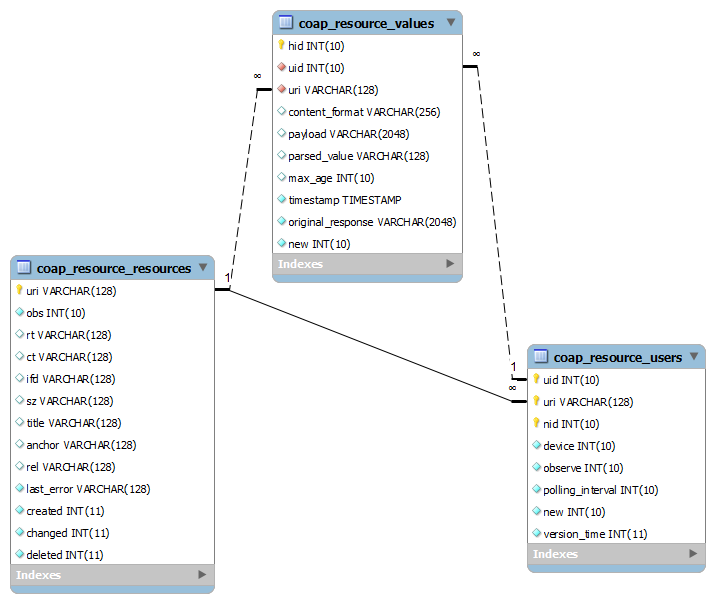
\includegraphics[width=1\textwidth]{fig/databankModel}
\caption{EER-diagram van de door ons toegevoegde tabellen}
\label{fig:databankModel}
\end{figure}

\subsubsection{coap\_sensor\_resource}
De tabel bevat informatie over CoAP-resources die toegevoegd werden aan de website. Hij bevat volgende kolommen (Zie figuur \ref{fig:databankModel}):
\begin{itemize}
\item uri: Dit is de volledige URI van de resource, dus IPv6-adres en URI-path. Dit is tevens de primaire sleutel van deze kolom, elke waarde moet dus uniek zijn.
\item obs, rt, ct, ifd, sz, title, anchor en rel: Deze kolommen bevatten waarden die bekomen worden bij resource disovery. Deze werden eerder uitgelegd in paragraaf \ref{resourceDiscovery}.
\item last\_error: Deze kolom bevat voor elke resource de laatst opgetreden fout. Zo kan een browser te weten komen bij \textit{polling} dat er iets foutliep bij communicatie met de betreffende resource.
\item created: De UNIX timestamp van de tijd waarop deze resource aangemaakt werd.
\item changed: De UNIX timestamp van de tijd waarop deze resource het laatst gewijzigd werd.
\item not\_in\_core: Een waarde om aan te geven of deze resource nog in de well-known/core zit van een \textit{device}.
\end{itemize}
\subsubsection{coap\_sensor\_interested\_user}
In deze tabel wordt bijgehouden welke gebruikers ge\"{i}nteresseerd zijn in specifieke resources en \textit{devices}. Hij bevat een entry voor elk koppel gebruiker/resource en gebruiker/\textit{device} en wordt impliciet geassoc\"{i}eerd met een instantie van respectievelijk coap\_resource of coap\_device. Op die manier kan per user worden bijgehouden wat hij/zij met een bepaalde resource wil doen. Ze bestaat uit de volgende kolommen:
\begin{itemize}
\item uid: Een unieke identificatie voor een gebruiker. Dit ID is overgenomen uit Drupal, daar hebben alle gebruikers ook een uniek user ID. Deze kolom is tevens deel van de primaire sleutel.
\item uri: De URI van de resource waarin de gebruiker ge\"{i}nteresseerd is. Dit is dezelfde URI als in de vorige tabel (coap\_resource\_resources). Deze kolom vormt dus een foreign key en maakt tevens deel uit van de primaire sleutel.
\item nid: Een unieke identificatie van de node (node ID)\nomenclature{nid}{Node ID} waaraan de resource gekoppeld is in Drupal. Deze kolom is ook deel van de primaire sleutel.
\item \textit{device}: Deze waarde geeft aan of het een resource of een volledig \textit{embedded device} betreft (0 = resource, 1 = \textit{device}).
\item \textit{observe}: Deze waarde geeft aan of de gebruiker momenteel de resource wil observeren of niet (0 = niet observeren, 1 = wel observeren).
\item \textit{polling\_interval}: Dit is de periode in seconden tussen twee polls van de browser naar de Drupal-server, deze is default drie seconden.
\item new: Deze waarde duidt aan of er inmiddels een nieuwe \textit{discovery} is uitgevoerd of bezig is voor een \textit{device}. Deze waarde heeft momenteel enkel nut voor \textit{devices}. (0 = up-to-date, 1 = \textit{discovery} bezig, 2 = \textit{discovery} klaar/referentiegegevens moeten geupdated worden)
\end{itemize}
De primaire sleutel bestaat uit de combinatie van de kolommen uid, uri en nid. Elke combinatie van waarden uit deze drie kolommen moet per entry uniek zijn.

\subsubsection{coap\_sensor\_value}
Deze tabel bevat een entry voor elke waarde die is binnengekomen. Bovendien wordt een nieuwe waarde even veel keren toegevoegd als er ge\"{i}nteresseerden zijn voor die waarde op dat moment. Dit lijkt op het eerste zicht redundante informatie, maar het heeft wel degelijk nut. Zo kan men bijvoorbeeld later te weten komen voor een bepaalde user, welke waarden hij/zij in welke periode heeft opgevraagd. Men zou als alternatief ook relaties kunnen leggen tussen waarden en users, zo hoeven er geen duplicaten van waarden opgeslagen te worden. De tabel bevat de volgende kolommen:
\begin{itemize}
\item hid: Een uniek ID voor de entry automatisch gegenereerd bij toevoegen aan de databank. Dit is de primaire sleutel, dus deze waarden moeten uniek zijn.
\item uid: Het ID van de user waarvoor deze waarde opgeslagen is. Dit is hetzelfde ID als in de coap\_resource\_users-tabel en vormt dus een foreign key.
\item uri: De URI van de resource waarvan deze waarde komt. Dit is dezelfde URI als in de coap\_resource\_resources-tabel en vormt dus een foreign key.
\item content\_format: Bevat voor elke entry het formaat van het bericht, aangeduid met een leesbare naam (bijvoorbeeld plain text, JSON, ...). 
\item payload: De payload van het bericht in leesbare vorm.
\item parsed\_value: Indien mogelijk bevat dit een waarde die geparset is uit de payload, bijvoorbeeld een numerieke waarde. Indien er geen waarde kon geparset worden bevat deze kolom gewoon de payload.
\item max\_age: Geeft aan wat de geldigheidsduur is voor deze waarde, deze is default nul.
\item timestamp: Het tijdstip waarop de waarde in de databank werd opgeslagen in mysql timestamp-formaat. Deze wordt automatisch gegenereerd. Samen met de \textit{max-age} kan men dus bepalen of de waarde nog geldig is.
\item original\_response: De originele response op het CoAP-\textit{request}bericht in hexadecimale vorm.
\item new: Geeft aan of de waarde reeds opgehaald werd om te tonen aan de gebruiker (0 = reeds opgehaald, 1 = nog niet opgehaald, default waarde = 0).
\end{itemize}

\newpage
\section{Contenttypes in Drupal}

Bij installatie van de module worden twee contenttypes mee ge\"{i}nstalleerd. We bespreken wat de mogelijkheden ervan zijn en hoe ze eruitzien. Het laten installeren van contenttypes zorgt ervoor dat een Drupal-gebruiker op een eenvoudige manier content kan toevoegen, in dit geval onderdelen van een CoAP-sensornetwerk. Concreet moet de gebruiker enkel op 'Add content' klikken op zijn/haar Drupal-website en het gewenste contenttype aanklikken. Na invullen van enkele vereiste velden wordt een node gecre\"{e}erd die de content voorstelt.
\begin{figure}[h!]
\vspace{10pt}
\centering
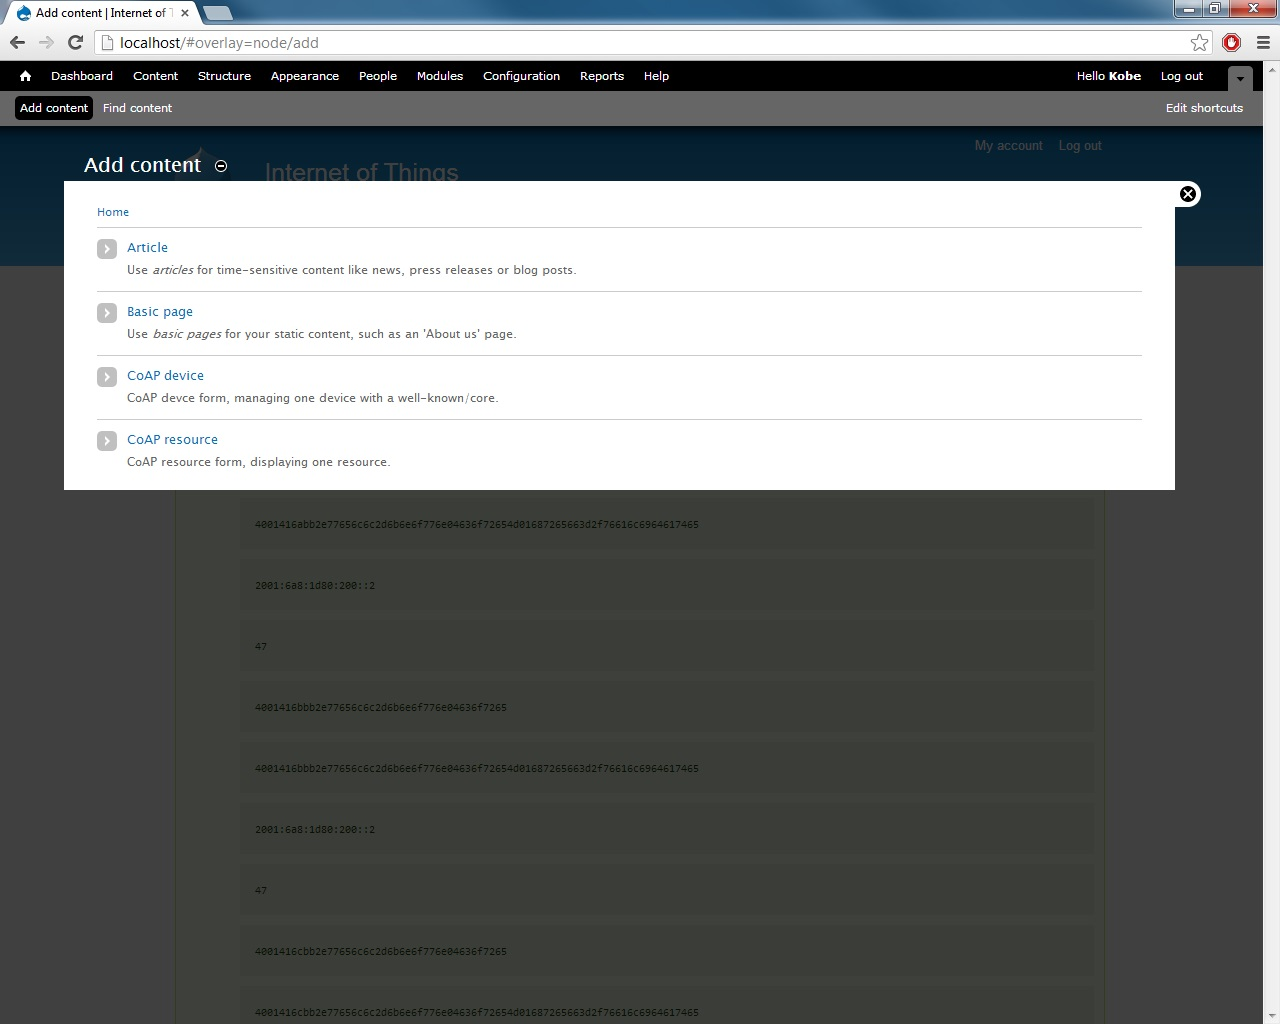
\includegraphics[width=1\textwidth]{fig/add_content}
\caption{Content toevoegen door op 'Add content' te klikken}
\label{fig:addContent}
\end{figure}

\newpage
\subsection{CoAP-resource}
\begin{wrapfigure}{r}{0.6\textwidth}
\vspace{-10pt}
%\hspace{-10pt}
\centering
\label{fig:addCoapResource}
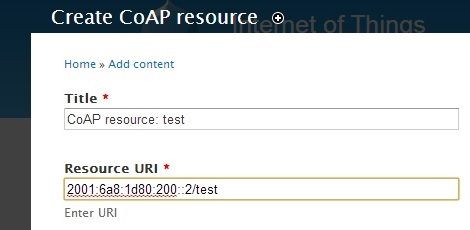
\includegraphics[width=0.6\textwidth]{fig/add_coap_resource}
\vspace{-20pt}
%\hspace{-10pt}
\centering
\caption{Adding content of contenttype CoAP-resource}
\centering
\vspace{-10pt}
\end{wrapfigure}
Dit contenttype stelt \'{e}\'{e}n resource voor. Bij het toevoegen wordt de URI opgegeven, deze bestaat uit het IPv6-adres van het \textit{embedded device} waarop de resource is aangesloten en een URI-path. IPv6-adres en URI-path worden gescheiden door een slash ('/'). Een voorbeeld van een door ons vaak gebruikte URI is: coap://2001:6a8:1d80:200::2/test. Vooraleer een resource effectief toegevoegd wordt, wordt hij gevalideerd. We voegen custom validatie toe via hook\_form\_alter. Indien de structuur van de URI niet geldig is of de resource al eerder door de gebruiker is toegevoegd, wordt er een foutmelding getoond en krijgt de gebruiker opnieuw de kans om een geldige/andere URI op te geven. Een andere manier om validatie van een veld te verwezenlijken is het maken van een custom veld met de Field API \cite{fieldAPI}. Op deze manier is de validatie onderdeel van het veld en hoeft ze niet achteraf toegevoegd te worden, wat gebeurt in hook\_form\_alter(). Deze methode gaf echter problemen indien content van dit type gewijzigd werd door middel van de \textit{Entity API}. Na een succesvolle validatie, wordt er content van het type coap\_resource toegevoegd. Door middel van hook\_node\_insert worden er enkele dingen in de databank toegevoegd. Er wordt een entry in de tabel coap\_sensor\_interested\_user toegevoegd waarmee wordt aangegeven dat de gebruiker die de resource toevoegde ge\"{i}nteresseerd is in de resource. Er wordt ook gekeken of er voor deze resource informatie beschikbaar is in de tabel coap\_sensor\_resource. Indien dit niet het geval is wordt een parti\"{e}le resource \textit{discovery} uitgevoerd voor die resource. Door middel van query filtering worden de opgehaalde gegevens toegevoegd aan de de databank. Indien er wel informatie beschikbaar is moet er niets meer gebeuren en krijgt de gebruiker de visuele representatie van de content te zien.\\

De gebruiker krijgt nu de kans om de REST-methodes  GET, PUT, POST en DELETE uit te voeren en een \textit{observe}. Bovendien krijgt de gebruiker een geschiedenis van opvragingen voor deze resource te zien en krijgt hij/zij ook de kans een grafiek te laten genereren. Voor het type grafiek heeft de gebruiker de keuze uit een lijn-, staaf-, of taartgrafiek. De gebruiker moet zelf weten welke soort grafiek nuttige informatie kan bevatten. In tegenstelling tot vorige versies wordt de visualisatie van content van het type CoAP-resource verzorgd door een template.
\begin{figure}[h!]
\centering
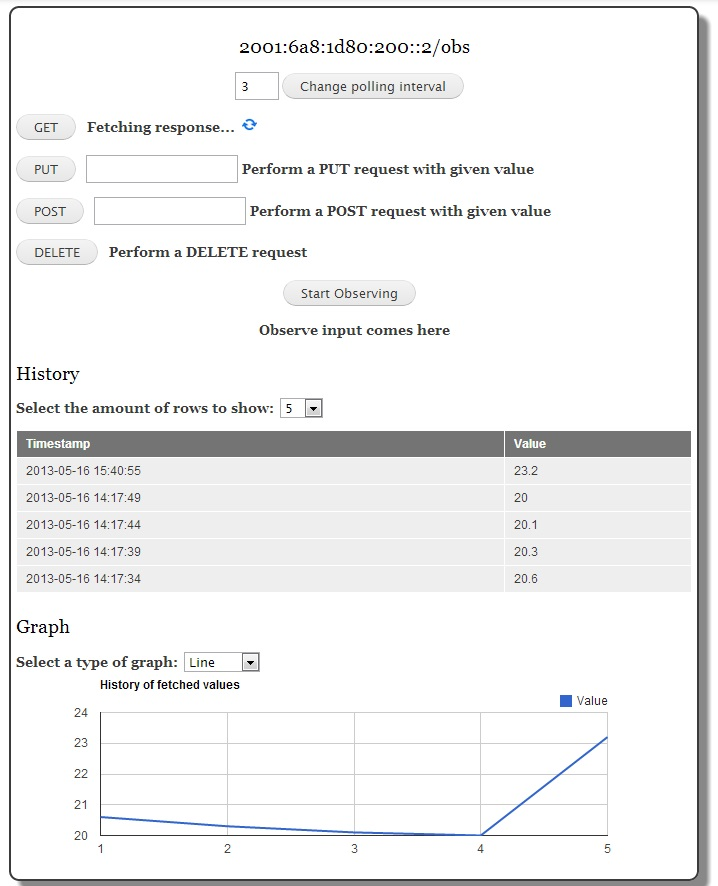
\includegraphics[width=0.7\textwidth]{fig/coap_resource}
\caption{Visuele representatie van het contenttype CoAP-resource}
\label{fig:coapResource}
\end{figure}

\subsubsection{Templating}\label{templating}
%Concreet maken we een template voor het contenttype CoAP-resource.
Drupal voorziet een handig mechanisme wanneer je een template voor een specifiek contenttype wil maken. Het enige wat men moet doen om ervoor te zorgen dat die template automatisch wordt opgeroepen voor het contenttype, is het template-bestand de juiste naam geven. Drupal voorziet namelijk in alle themes een standaard template voor een node, namelijk node.tpl.php. Om nu onze template te defini\"{e}ren, moet deze de naam node--coap\_resource.tpl.php dragen, daar de naam van ons contenttype coap\_resource is.\\

Het voordeel van deze benadering is dat de view gescheiden wordt van de rest van de code. Wanneer men bepaalde attributen of content nodig heeft voor de visuele representatie, kan men die variabelen voorzien door gebruik te maken van hook\_preprocess\_node(). Deze \textit{hook} wordt op voorhand opgeroepen en variabelen worden klaargezet. In het template-bestand kan men deze variabelen bereiken aan de hand van PHP-scriptlets (Zie listing \ref{template}). Men kan in deze templates dus ook PHP-code laten uitvoeren, al beperkt men dit best tot een minimum om de view gescheiden te houden. Zo wordt bij ons de URI van de resource en enkele waarden gebruikt in het template-bestand. Voor de rest bevat het template-bestand vooral HyperText Markup Language (HTML) \nomenclature{HTML}{HyperText Markup Language} om de gegevens te visualiseren.\\

Er stelt zich nu wel nog een probleem, het template-bestand moet namelijk op de juiste plaats staan, en dit in de directory van het gebruikte theme. Men voegt echter beter geen bestanden toe aan de Drupalcore en bovendien kunnen wij dat ook niet verwachten van de eindgebruiker. Het template-bestand zou automatisch moeten worden opgenomen in het gebruikte theme, waarbij het template-bestand gewoon in onze module kan blijven staan. Na grondig onderzoek bleek dit mogelijk aan de hand van hook\_theme\_registry\_alter(). Deze \textit{hook} geeft ons de kans een pad toe te voegen aan het theme-registry, waardoor het template zal gevonden worden bij het bouwen van de view \cite{addTemplate}.

\lstset{language=HTML}
\begin{lstlisting}[label=template,caption=Voorbeeld van een template met PHP-scriptlets (node.tpl.php)]
<div id='node-<?php print $node->nid; ?>' >
	<?php print render($title_prefix); ?>
	<?php if (!$page): ?>
	<h2<?php print $title_attributes; ?>>
		<a href='<?php print $node_url; ?>'>
			<?php print $title; ?>
		</a>
	</h2>
	<?php endif; ?>
	<?php print render($title_suffix); ?>
</div>
\end{lstlisting}

\noindent

\subsubsection{Polling}\label{polling}
In vorige versies van de module had de gebruiker niet de kans om meerdere resources op \'{e}\'{e}n pagina te zetten met de \textit{Views}module. Dit was in principe wel mogelijk, maar er zouden fouten optreden daar de \textit{polling} gebeurde op basis van welke resource geselecteerd was. Dit selecteren van resources is in deze versie weggewerkt, elke resource is een op zichzelf staand geheel (Zie figuur \ref{fig:coapResource}). In deze laatste versie is dit wel mogelijk omdat het \textit{polling} mechanisme grondig werd aangepast zoals nu zal blijken.\\

Een poll gebeurt nu specifiek voor een URI die opgegeven wordt in de URL waarnaar een \textit{AJAX call} wordt uitgevoerd. Bovendien werd in de databank een extra kolom 'New' toegevoegd aan de waardentabel. Deze duidt aan of een waarde reeds is opgehaald of nog niet (0 = reeds opgehaald, 1 = nog niet opgehaald). De kolom heeft als default waarde 1, dus nieuwe waarden worden automatisch als nieuw aangeduid. Wanneer een waarde opgehaald wordt uit de databank wordt de waarde in de kolom 'New' op 0 gezet.\\
Het pollen naar waarden voor een specifieke URI gebeurt nu als volgt:
\begin{itemize}
\item Er wordt in jQuery een \textit{AJAX call} uitgevoerd naar een bepaalde URL, bijvoorbeeld http://localhost/coap\_resource/poll/2001:6a8:1d80:200::2\textbar test. In de URI wordt een slash vervangen door een rechte streep ('\textbar'), anders wordt de slash ge\"{i}nterpreteerd.
\item Op de webserver wordt in Drupal de URI uit de aanvraag-URL gehaald en worden de slashes terug geplaatst.
\item De URI wordt gebruikt in een select-query om de nog niet opgehaalde waarden op te halen, dit wil zeggen de rijen waarvan de waarde in de kolom 'New' op 1 staat.
\item Er wordt een update-query uitgevoerd om van de opgehaalde rijen de waarde in de kolom 'New' te wijzigen naar 0. Dit om aan te geven dat de waarden reeds opgehaald werden.
\item De opgehaalde rijen worden in een XML-structuur gegoten samen met identificatie van de resource (de URI) en een eventuele errorstring. Deze XML-structuur wordt na deze stappen toegelicht.
\item De XML-structuur wordt uitgeprint en dus teruggestuurd als antwoord op de \textit{AJAX call}.
\item in jQuery wordt dan het antwoord geparsed. De errorstring wordt eruit gehaald en eventuele fouten worden getoond aan de gebruiker (Zie paragraaf \ref{foutmechanisme}). Daarna wordt elke opgehaalde rij \'{e}\'{e}n voor \'{e}\'{e}n overlopen en toegevoegd aan de visuele content die de gebruiker ziet.
\end{itemize}

De XML-structuur die eerder werd aangehaald bestaat uit een allesomvattend hoofdelement \textless poll\textgreater. Dit element bevat 3 andere soorten elementen:
\begin{itemize}
\item \textless uri\textgreater: Dit element komt \'{e}\'{e}n keer voor, het bevat de URI en dus de identificatie van de resource.
\item \textless error\textgreater: Net als het vorige element komt dit element ook \'{e}\'{e}n keer voor, het bevat de eventuele errorstring. Deze kan \'{e}\'{e}n van de volgende zijn: none, delay, broken of unreachable.
\item \textless entry\textgreater: Dit element stelt een rij voor met een waarde. Dit element kan dus nul of meer keren voorkomen. Het bestaat zelf uit de volgende elementen:
\begin{itemize}
\item \textless Hid\textgreater: de history ID van de rij.
\item \textless Value\textgreater: de effectieve (eventueel geparsete) waarde van de rij.
\item \textless \textit{Max age}\textgreater: Het aantal seconden dat deze waarde als geldig mag worden beschouwd.
\item \textless \textit{Timestamp}\textgreater: Het tijdstip waarop de waarde ontvangen werd op de Drupal-server.
\end{itemize}
\end{itemize}

Een voorbeeld van een antwoord op een \textit{AJAX call} bij \textit{polling}:

\lstset{language=XML}

\begin{lstlisting}[label=xmlPolling,caption=Voorbeeld antwoord op \textit{AJAX call} bij polling]
<poll>
	<uri>2001:6a8:1d80:200::2</uri>
	<error>none</error>
	<entrys>
		<entry>
			<hid>76</hid>
			<value>20.2</value>
			<max_age>30</max_age>
			<timestamp>2013-05-20 20:36:32</timestamp>
		</entry>
		<entry>
			<hid>77</hid>
			<value>20.4</value>
			<max_age>30</max_age>
			<timestamp>2013-05-20 20:36:37</timestamp>
		</entry>
	</entrys>
</poll>
\end{lstlisting}

\subsubsection{Foutmechanisme} \label{foutmechanisme}
Tot nog toe bleef de gebruiker in het ongewisse wanneer er iets foutliep in de communicatie met een CoAP-resource. Dit is niet gebruiksvriendelijk en kan voor ergernissen zorgen.\\
Nu hebben we in de vorige hoofdstukken al gezien dat fouten al geregistreerd worden aan de hand van enkele errorstrings. Deze zijn zelfs al ter beschikking in jQuery bij elke poll (Zie \textit{polling} hierboven). Het enige wat nu nog moet gebeuren is een gepaste boodschap tonen in de visuele representatie. Zoals te zien in figuur \ref{fig:foutmechanisme} wordt in het groen een vinkje getoond wanneer een operatie geslaagd is. Wanneer de communicatie niet gelukt of foutgelopen is wordt de methode geannuleerd en wordt een kruisje in het rood getoond. Ook wanneer een methode niet ondersteund is, wordt dit kruisje getoond. Wanneer het antwoord op zich laat wachten worden roterende blauwe pijltjes getoond.

\begin{figure}[h!]
\centering
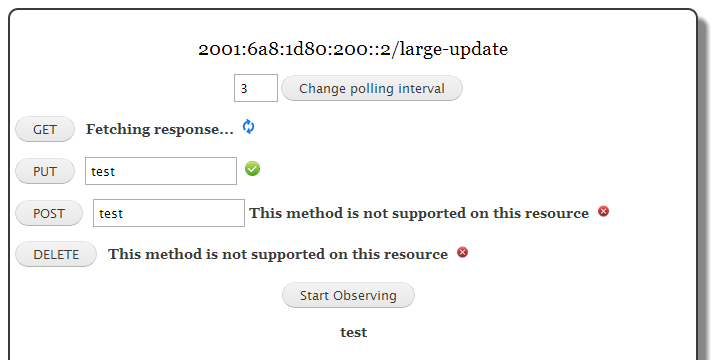
\includegraphics[width=1\textwidth]{fig/foutmechanisme}
\caption{Mechanisme om fouten te tonen aan de gebruiker}
\label{fig:foutmechanisme}
\end{figure}

\newpage
\subsection{CoAP-device}
\begin{wrapfigure}{r}{0.6\textwidth}
\vspace{-10pt}
%\hspace{-10pt}
\centering
\label{fig:addCoapDevice}
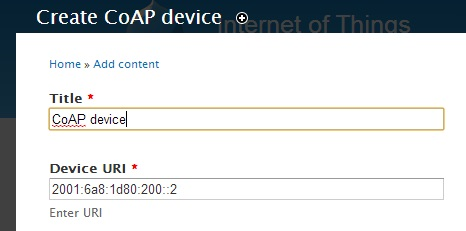
\includegraphics[width=0.6\textwidth]{fig/add_coap_device}
\vspace{-20pt}
%\hspace{-10pt}
\centering
\caption{Adding content of contenttype CoAP-device}
\centering
\vspace{-20pt}
\end{wrapfigure}
Dit contenttype stelt een volledig \textit{embedded device} voor waarop zich \'{e}\'{e}n of meerdere resources bevinden. Bij toevoegen van dit contenttype hoeft de gebruiker enkel het IPv6-adres op te geven in het veld field\_device\_uri. Er is nog een veld aanwezig in dit contenttype, namelijk het veld field\_resource\_references. Dit veld is onzichtbaar bij het aanmaken of wijzigen van content zodat een gebruiker dit veld niet kan aanpassen. Het mag enkel vanuit code aangepast worden en bevat referenties naar content van het type CoAP-resource die overeen komt met de resources uit de well-known/core van het \textit{device}.\\

Net zoals bij CoAP-resource voegen we custom validatie voor het URI-veld toe via hook\_form\_alter. De structuur van de URI moet bestaan uit een IPv6-adres en de gebruiker mag het \textit{device} niet eerder toegevoegd hebben. Ook hier stoppen we extra gegevens in de databank via hook\_node\_insert. Er wordt een entry in de tabel coap\_sensor\_interested\_user toegevoegd waarmee wordt aangegeven dat de gebruiker ge\"{i}nteresseerd is in het \textit{device}. Deze tabel heeft een kolom om aan te geven dat de entry verwerkt moet worden. Deze kolomwaarde is afhankelijk van het feit of er andere gebruikers ge\"{i}nteresseerd zijn in het \textit{device} op het moment dat dit \textit{device} toegevoegd wordt. Als dit het geval is hoeven we geen resource \textit{discovery} voor dit \textit{device} uit te voeren en wordt als kolomwaarde het getal 2 gebruikt. We zijn immers zeker dat alle resourcegegevens al in de databank zitten. Indien niemand ge\"{i}nteresseerd is in het \textit{device} wordt als kolomwaarde het getal 1 gebruikt en wordt een resource \textit{discovery} uitgevoerd. Na het toevoegen van het \textit{device} krijgt de gebruiker de visuele representatie van de content te zien.\\

De visuele representatie gebeurt hier niet met een template maar door gebruik te maken van een form \cite{formAPI}. Wanneer de pagina galaden is, start een periodieke poll vanuit jQuery naar de \textit{callback}functie coap\_device\_page\_callback(). In deze functie wordt de rij die overeenkomt met het toegevoegde \textit{device} uit de tabel coap\_sensor\_interested\_user gehaald. Afhankelijk van de kolomwaarde 'new' gebeuren er enkele zaken. Indien 'new' de waarde 0 heeft, is de output van deze \textit{callback}functie een lege string en gebeurt er verder niks. Bij de waarde 1 heeft de functie als output 'show\_counter'. Bij elke poll vanuit jQuery waar de functie 'show\_counter' als output heeft, wordt een teller verhoogd. Afhankelijk van deze teller wordt er een boodschap getoond op de pagina. Op deze manier heeft de gebruiker feedback indien de resource \textit{discovery} langer duurt dan normaal. Een voorbeeld zie je op figuur~\ref{fig:coapDeviceMessage}.
\begin{figure}[h!]
\centering
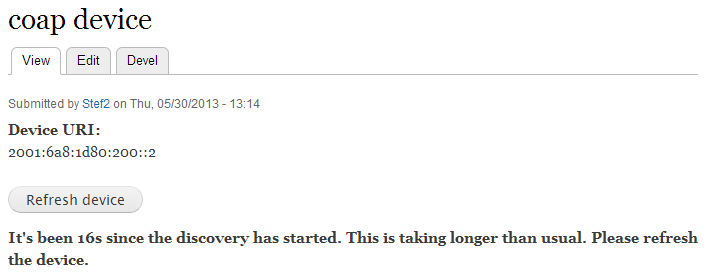
\includegraphics[width=1\textwidth]{fig/CoAPDeviceMessage}
\caption{Variabele boodschap bij content van type CoAP-device}
\label{fig:coapDeviceMessage}
\end{figure}

\noindent
In het geval 'new' de waarde 2 bevat, moet field\_resource\_references geupdated worden. Alle referenties in het veld worden verwijderd en de nieuwe lijst van referenties wordt op volgende manier opgebouwd. De gegevens van de resources in de well-known/core worden opgehaald uit de coap\_sensor\_resourcetabel en voor elke resource wordt gekeken of de gebruiker al ge\"{i}nteresseerd is in deze resource. Als dit zo is hoeft er enkel een referentie aangemaakt te worden naar deze resource want een gebruiker mag een resource maar \'{e}\'{e}n keer toevoegen. Als dit niet het geval is moet er content van het type CoAP-resource aangemaakt worden. Zoniet kan er geen referentie naar deze content toegevoegd worden. Er zijn twee aanvaardbare manieren om content toe te voegen, namelijk door gebruik te maken van node\_save() en dergelijke specifieke functies voor nodes of door gebruik te maken van de \textit{Entity API}. Deze laatste manier heeft de voorkeur omdat de aangeboden functies van de \textit{Entity API} generiek zijn en op alle soorten entities werken. De node-specifieke functies werken enkel op nodes.\\

Als het veld ge\"{u}pdated is heeft de \textit{callback}functie 'reload' als output. Wanneer deze string herkend wordt in jQuery wordt de pagina herladen. Na het herladen zie je dat het veld field\_resource\_reference een lijst van referenties bevat. Nu kan de gebruiker doorklikken naar een resource naar keuze. Wanneer de gebruiker die het \textit{device} toevoegde deze content bekijkt, heeft hij de mogelijkheid de \textit{discovery data} te vernieuwen door een nieuwe resource \textit{discovery} uit te voeren. Alle content die overeenstemt met dit \textit{device} wordt geupdated bij de volgende jQuery-poll wanneer ze weergegeven worden. De mogelijkheid om een nieuwe resource \textit{discovery} uit te voeren voor een \textit{device} is enkel beschikbaar voor de gebruiker die het \textit{device} toevoegde. Dit om anonieme gebruikers geen kans te geven het \textit{device} te overspoelen met resource discoveries.
\begin{figure}[h!]
\centering
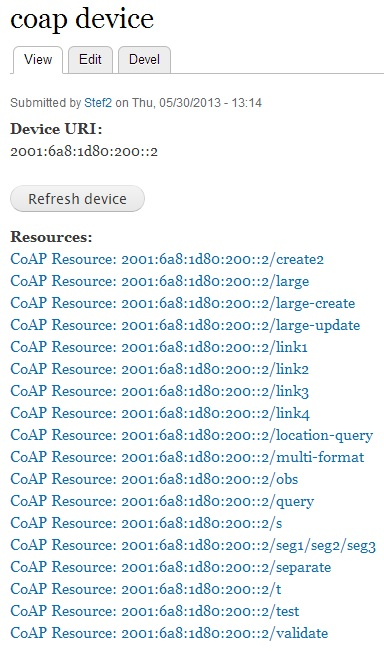
\includegraphics[width=0.6\textwidth]{fig/coap_device}
\caption{Visuele representatie van het contenttype CoAP-device}
\label{fig:coapDevice}
\end{figure}

%hier moet alles komen
%it wordt gerealiseerd met de al eerder behandelde contenttypes. Er worden nu twee contenttypes gecre\"{e}erd bij installatie van de module, \'{e}\'{e}n voor een CoAP-resource (Zie figuur \ref{fig:coapResource}) en \'{e}\'{e}n voor een CoAP-device (Zie figuur \ref{fig:coapDevice}).\\

%Wanneer een CoAP-device wordt toegevoegd door de gebruiker, wordt er automatisch een resource \textit{discovery} op uitgevoerd. De gebruiker krijgt dan een lijst van links te zien, \'{e}\'{e}n link per aangesloten CoAP-resource (Zie figuur \ref{fig:coapDevice}). Bovendien wordt voor elk van die resources content aangemaakt van het contenttype CoAP-resource. De gebruiker zal geen 2 gelijke resources kunnen toevoegen om duplicatie van content te vermijden. Wanneer de gebruiker toch dezelfde resource op verschillende plaatsen van de website wil krijgen, raden wij aan de \textit{Views}module te gebruiken \cite{viewsModule}. Met \textit{Views} kan men meerdere visuele representaties maken van dezelfde content, dus zonder content te dupliceren.

\section{Implementatie van de CoAP-libraryhooks}
In deze paragraaf bekijken we hoe deze module de \textit{hooks} implementeert die de CoAP-\textit{library} voorziet (Zie paragraaf \ref{observe_hooks}).

\subsection{hook\_receive\_notification()}
Deze \textit{hook} wordt opgeroepen door de CoAP-\textit{library} wanneer een bericht binnenkomt op de socket. Er wordt een response-object gemaakt van de klass CoAPMessage dat tevens meegegeven wordt als enige attribuut van de \textit{hook}.\\
In deze module worden in de \textit{hook} volgende stappen ondernomen:
\begin{itemize}
\item De benodigde waarden worden uit het response-object gehaald en in de databank gestopt voor de huidige gebruiker.
\item De user ID's van alle andere ge\"{i}nteresseerden (dus niet de huidige gebruiker) voor de betreffende resource worden opgehaald uit de databank.
\item Voor elk van deze gebruikers worden de waarden uit het response-object ook toegevoegd aan de databank.
\end{itemize}

\subsection{hook\_receive\_error()}
Deze \textit{hook} wordt voorzien van de volgende parameters: een errorstring, het IPv6-adres van het \textit{embedded device} en de naam van de resource. Ze wordt opgeroepen wanneer \'{e}\'{e}n van de volgende gebeurtenissen zich voordoet:
\begin{itemize}
\item De socket kon niet worden geopend naar het \textit{embedded device}. Deze gebeurtenis resulteert in een errorstring gelijk aan 'unreachable'.
\item De tijdsspanne verstrijkt waarin een antwoord zou moeten ontvangen zijn, dit wordt bepaald met het exponential backoff-mechanisme (Zie paragraaf \ref{exponentialBackoff}). Dit levert een errorstring gelijk aan 'delay'.
\item Het maximum aantal pogingen om het bericht opnieuw te versturen is verstreken (Zie paragraaf \ref{exponentialBackoff}). Nu zal de errorstring gelijk zijn aan 'broken'.
\item Ook wanneer het zeker is dat er geen fout is opgetreden, wordt dit gemeld met deze \textit{hook}. De errorstring wordt dan gelijk aan 'none'.
\end{itemize}
Wanneer nu de \textit{hook} wordt opgeroepen voor de module die in dit hoofdstuk besproken wordt, zal de errorstring opgeslagen worden bij de betreffende resource in de databank.

\subsection{hook\_stop\_observers()}
Wanneer een \textit{observe} moet be\"{e}indigd worden, om welke reden dan ook (bijvoorbeeld wanneer de resource niet meer te bereiken is), wordt deze \textit{hook} opgeroepen. Men moet hier echter wel opletten, want de resource kan zich in een soort slaaptoestand bevinden. De resource lijkt dan onbereikbaar, maar deze zal nog steeds notificaties sturen.\\
De hook krijgt als parameters het IPv6-adres van het \textit{embedded device} en de naam van de resource mee. Zo kan de module die deze \textit{hook} implementeert ervoor zorgen dat de toestand consistent blijft voor de andere gebruikers.\\
Concreet zal de module die in dit hoofdstuk wordt besproken, in de databank aanduiden dat gebruikers de betreffende resource niet meer aan het observeren zijn. Dit wordt voor elke user gedaan die ge\"{i}nteresseerd was in deze resource.